\documentclass[letterpaper]{article}
\usepackage[bottom=1.1in,top=0.9in,left=1.15in,right=1.15in]{geometry}
\usepackage[english]{babel}
\usepackage[utf8x]{inputenc}
\usepackage[T1]{fontenc}
\usepackage{amsmath}
\usepackage{amsfonts}
\usepackage{bm}
\usepackage[square,sort,comma,numbers]{natbib}
\usepackage{graphicx}
\usepackage[colorinlistoftodos]{todonotes}
\usepackage[colorlinks=true, allcolors=blue]{hyperref}
\usepackage[titletoc,title]{appendix}
\usepackage{authblk}
\usepackage[linesnumbered,ruled]{algorithm2e}

\newcommand{\cp}{^c}
\newcommand{\df}{\mathrm{d}}
\newcommand{\dm}{\mathcal{D}}
\newcommand{\fc}[1]{\sigma^2(#1)}
\newcommand{\id}[1]{\mathbb{I}\{#1\}}
\newcommand{\prob}{\mathbb{P}}
\newcommand{\XX}{\mathbf{X}}
\newcommand{\YY}{\mathbf{Y}}
\newcommand{\ZZ}{\mathbf{Z}}
\newcommand{\Ee}{\bm{\epsilon}}
\newcommand{\Rr}{\mathbf{r}}
\newcommand{\Mo}{\bm{\mu_1}}
\newcommand{\Mt}{\bm{\mu_2}}
\usepackage[english]{babel}

\usepackage{xcolor}
\definecolor{verde}{rgb}{0.25,0.5,0.35}
\definecolor{jpurple}{rgb}{0.5,0,0.35}
\definecolor{darkgreen}{rgb}{0.0, 0.2, 0.13}
\usepackage{listings}


\title{Markov Chain Monte Carlo Simulation on\\Stochastic Volatility Estimation of S\&P500 Returns}
\author{
	Kapil Kanagal\\ \texttt{kkanagal@stanford.edu}
	\and
	Lorenzo Limonta\\ \texttt{llimonta@stanford.edu}
	\and	
	Quan Chen\\ \texttt{quanchen@stanford.edu}
	\and
	Jiacheng Zou\\ \texttt{jasonzou@stanford.edu}
}
\author{
	Kapil Kanagal\qquad Lorenzo Limonta\qquad Quan Chen \qquad Jiacheng Zou
	\\\texttt{\{kkanagal,llimonta,quanchen,jasonzou\}@stanford.edu}
}


\begin{document}
	\maketitle
	\tableofcontents
	\newpage
	\begin{abstract}
		This paper seeks to explore the applications of Markov Chain Monte Carlo techniques on  S\&P 500  data in order to estimate latent volatility. The model used is a stochastic volatility model originally proposed by \citet{rossi1994bayesian}, which uses an AR(1) parametrization for the conditional variance of the return. The model's parameters are fitted on the daily return (Jan 2003 - Dec 2012) by using as explanatory variables the lagged-1 return. The mean squared error obtained is approximately 0.42 with an arbitrarily early stopping condition $R^2=80\%$, otherwise within 100 iterations MCMC would reach a $R^2=100\%$ thus over-fitting towards the data. We formulate our model in a very generic way so that we can improve robustness by easily changing the priors without changing the updating schemes, and we can add in jump terms or other exogenous covariates without changing the mathematical formulations.
	\end{abstract}
	\section{Introduction}
	Markov Chain Monte Carlo (MCMC) is a commonly used technique for estimating by simulation the expectation of a statistic in a complex model. Successive random selections form a Markov chain, the stationary distribution of which is the target distribution. It is particularly useful for the evaluation of posterior distributions in complex Bayesian models. In the Metropolis–Hastings algorithm, items are selected from an arbitrary “proposal” distribution and are retained or not according to an acceptance rule. The Gibbs sampler is a special case in which the proposal distributions are conditional distributions of single components of a vector parameter \cite{gilks2005markov}.
	
	This has become a commonly used technique to sample from a complicated distribution. Often times, the parameters in a distribution are unknown and resultantly, this makes it extremely difficult to draw from the given distribution. MCMC can be used to estimate these parameters in order to give a clearer picture of the properties of the distribution. This technique combines two other techniques (Markov Chains and Monte Carlo Simulation) to solve this problem.
	
	\subsection{Markov Chains}
	
	By definition, a Markov Chain is a stochastic model describing a sequence of possible events in which the probability of each event depends only on the state attained in the previous event. These mathematical systems move from one state to another in the state space -- a list of all possible states. With a two state model (states A and B), there are a possible four transitions. A->B, B->A, A->A, B->B. Each move in the Markov Chain is called a step. Instead of using a visual diagram to represent the Markov Chain, a transition matrix is used to tally all the potential transition properties. This allows for all sorts of unique linear algebra usages of these matrices, which can be used to describe even more complex state spaces.\cite{grinstead1997}
	
	The interesting part of MCMC, is that random walks (i.e. Brownian Motion) can be modeled as Markov Chains. This creates a unique instance, which allows MCMC to model a variety of interesting problems in statistics, biology, physics, and finance. In finance, random walks are often use to model stochastic volatility and pricing models. Below is a simple example of a Markov Chain to give you some intuition for their structure. Recall that the problem we’re trying to solve is to draw from a distribution over a finite set X with probability function p(x). The MCMC method is to construct a Markov chain whose stationary distribution is exactly p, even when you just have black-box access to evaluating p.
	\begin{center}
		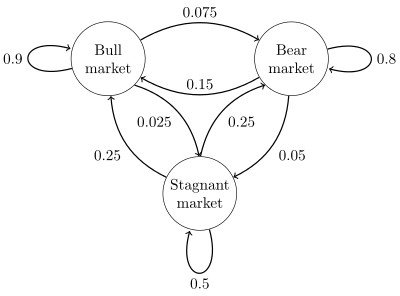
\includegraphics[scale=0.4]{Markov_Chain.png}
	\end{center}
	\subsection{Monte Carlo Simulation}
	
	The Monte Carlo part of MCMC refers to the simulation portion of the process. Monte Carlo simulation generates a large number of simulated outcomes, from which an average or a probability is estimated. A simple example would be to use Monte Carlo simulation to estimate the probability of a coin toss landing heads ten times in a row. Simulate ten coin tosses, observe if you get ten heads in a row, and repeat this simulation, 1 million times (or a large number of times). Out of these 1 million simulations, let's say you observed 967 instances in which you observed ten heads in a row, which means that the probability of getting ten heads in a row is about 967 / 1000000 $\times$ 100 = 0.0967\%. Calculating the result mathematically as opposed to using Monte Carlo simulation, we get: $0.5^{10}$ = 0.00097656 = 0.0977\%.
	
	
	
	Thus, MCMC uses Monte Carlo Simulations on Markov Chains to determine the distribution from which the parameters are drawn and estimate averages for the sample parameters. It does so for each transition in the Markov Chain process that is generated. Now that we have established an understanding of both MC parts (Markov Chains and Monte Carlo Simulation) work, we use the sections below to outline a more rigorous mathematical background of MCMC, followed by our empirical MCMC simulations run on S\&P 500 data. Be sure to remember, that the core problem MCMC tries to solve is a sampling problem.
	
	%\newpage
	\section{Bayesian Statistics}
	\subsection{Preliminaries}
	The entire mathematical argument upon which MCMC is predicated on, is the use of Bayesian inference: the ability to combine prior beliefs with data, in order to compute the posterior distribution and make inferences on an event \cite{tsay2002}. Bayesian inference is about the quantification and propagation of uncertainty, defined via a probability, in light of observations of the
	system. Unlike the frequentist approach, Bayesian statistics models both the data and the parameters that govern the model to be probabilistic. 
	Any event that can be witnessed or recorded, occurs under some specific conditions which may (or may not) be observed. Bayesian statistics tries to define the probability of an event E, given some hypothesis H that describes the condition under which E may happen.  \\
	The following four axioms make for the building blocks of Bayesian statistics \cite{lee2012bayesian}:
	\begin{equation}
	P(E|H) \geq 0 \qquad \text{for all E,H}
	\label{eq:Ax1} 
	\end{equation}
	\begin{equation}
	P(H|H) = 1 \qquad \text{for all H}
	\label{eq:Ax2}
	\end{equation}
	\begin{equation}
	P(E \cup F |H) = P(E|H) + P(F|H) \qquad \text{when E $\cap$ F  $\cap$ H} = \emptyset 
	\label{eq:Ax3} 
	\end{equation}
	\begin{equation}
	P(E|F\cap H) = \frac{P(E \cap F|H)}{P(F|H)}
	\label{eq:Ax4} 
	\end{equation}
	
	Defining $|$ as a conditional probability, we have that eq. \ref{eq:Ax1} tells us the probability of event E happening under condition H. $P(E|H)$ need be equal or greater than zero, since an event may or may not happen.
	Equation \ref{eq:Ax2} is the tautological condition: under hypothesis H, the probability of H happening must be 1. From a combination of eq. \ref{eq:Ax1},\ref{eq:Ax2} we can demonstrate that the probability of P(E|H) is between zero and one. Equation \ref{eq:Ax3} tells us that the probability of a specific set of events happening ($E\cup F$), given condition H, will be the sum of those events happening independently under condition H, iff the intersection between each set is empty. In lay terms, eq. \ref{eq:Ax3} tells us that the probability of a dicer to roll either a one or a two is equal to the probability of the dicer to roll one plus the probability of the dicer to roll two. Equation \ref{eq:Ax4} relates the probability of E happening given the union between two condition F and H.\\ \newline
	Given equations \ref{eq:Ax1}-\ref{eq:Ax4} we can obtain Bayes' theorem:
	
	\begin{equation}
	P(H|E)=\frac{P(E|H)\cdot P(H)}{P(E)}
	\end{equation}
	
	which allows to compute the posterior distribution given information on the prior. \begin{enumerate}
		\item P(H) is defined as the prior probability, i.e. the estimate of the probability of hypothesis H before the data E, our evidence, is observed.
		\item P(E|H) is the probability of observing E given H. It indicates the compatibility of the evidence with the given hypothesis.
		\item P(E) is defined as the marginal likelihood or "model evidence".
		\item P(H|E) is termed as the posterior probability, i.e. the probability of H given our observations E. This is what we want to know: the probability of a hypothesis given the observed evidence.
	\end{enumerate} 
	
	Bayes' theorem is usually proposed in the following manner
	
	\begin{equation}
	P(H|E) \propto P(H)P(E|H)
	\end{equation}
	
	This happens because the constant of proportionality $\frac{1}{P(E)}$ is generally intractable. Nonetheless, no loss of generality is introduced by doing this simplification.
	
	\subsection{Application to modeling}
	
	Having introduced the fundamental principle at the basis of Bayesian statistic, we want to extend its role to the solution of real world problems. 
	In almost all the situation we can think of, we are interested in estimating some k unknown quantities that make up our model M, where M is used to explain the data collected.\\
	Our k unwknown parameters will be called the theta vector
	$\vec{\Theta}$
	\begin{equation*}
	\textbf{ $\Theta$ } = \{ \theta_1 .... \theta_k \}
	\end{equation*}
	Meanwhile, the set of observed data relevant to estimate these parameters will be the set
	\begin{equation*}
	\textbf{Y}=\{y_1...y_n\}
	\end{equation*}
	
	Since we assume that our model predicts the n-observed data, our unknown parameters \textbf{$\theta$} must be related to our observations. Looking at our definition of Bayesian statistic, this dependence can be expressed as follows:
	\begin{equation}
	p(\textbf{$\Theta$}|\textbf{Y})
	\label{eq:StatsBayProb}
	\end{equation}
	Equation \ref{eq:StatsBayProb} simply tells us that we can attach a distribution to the values of our parameters under the hypothesis of having observed the \textbf{Y} data. By applying Bayes' theorem we can re-write the previous expression in familiar terms
	\begin{equation}
	p(\textbf{$\Theta$}|\textbf{Y}) \propto p(\textbf{$\Theta$})p(\textbf{Y}|\textbf{$\Theta$})
	\label{eq:BaePost}
	\end{equation}
	
	We have now simplified our problem.. To infer our posterior we simply need the prior distribution, i.e. our belief on what is the distribution of the parameters that need to be estimated, as well as being able to express the likelihood, i.e. the direct relationship for Y, fixed $\Theta$.
	
	\subsection{The prior distribution}
	A fundamental aspects of Bayesian statistics, and one of its inherent weaknesses, is the influence of the prior distribution on our solution. As clearly evidenced by eq. \ref{eq:BaePost}, the prior enters the posterior. The choice of the prior cannot be uniquely determined a priori, but are otherwise determined subjectively according to the beliefs of the practitioner \cite{gelman2008}. We will show that under certain conditions this inherent flaw of Bayesian statistics can be voided. Nonetheless, the prior plays an important role within Bayesian structure, it allows us to incorporate non-sample information (e.g. data from the existing literature) in a consistent manner. For example, in the context of econometrics, the prior provides a consistent mechanism to impose important information on certain parameters, such as positivity of volatility. It can impose stationarity, rule out near unit-root behavior, or separate mixture components \cite{johannes2003}. 
	
	When determining a prior distribution two key issues need to be taken into considerations
	
	\begin{itemize}
		\item what  information  is  going  into  the  prior  distribution
		\item the  properties  of  the  resulting  posterior  distribution
	\end{itemize}
	
	With well-identified parameters and large sample sizes,  prior  distributions can be reasonably chosen, and will have minor effects on posterior inferences since the likelihood will have a predominance on forming the posterior distribution \footnote{ We refer the reader to http://faculty.washington.edu/kenrice/BayesIntroClassEpi515.pdf for a visualization of this assertion} \cite{gelman2002}. If the sample size is small, or available data provide only indirect information about the parameters of interest,  the  prior  distribution  becomes  more  important.
	
	We can broadly distinguish three classes of priors \cite{gelman2002}:
	
	\begin{enumerate}
		\item Non-informative Prior Distributions
		\item Moderately Informative Hierarchical Prior
		Distributions
		\item Highly Informative Prior Distributions
	\end{enumerate}
	
	Class 1 is used in situation where there is no reasonable or intuitive knowledge about the parameter that need to be evaluated. Usually they corresponds to wide, flat distribution. Class 3 priors are parameters that have a substantial literature with established values and boundaries. Class 2 parameters, are parameters whose values are not well known, but have an established relationship. \\
	\indent Given this classification, one could be enticed into using non-informative prior for all parameters of the model of interest, in order to obviate to Bayesian's flaw. We strongly admonish against this practice. As noted in the opening paragraph of this section, the prior is used to provide constraints on the values that a specific parameter may assume, given existing accepted knowledge. Failing to make use of this information may lead to absurd estimation. \citet{gelman2002} in one such experiment of using only non-informative prior, evaluated the weight of the liver of his sample patients to be five to ten times those expected in literature.
	
	\subsection{The likelihood}
	In order to complete the definition of a Bayesian model, both the prior distributions and the likelihood must be approximated or fully specified.  The likelihood, likelihood function, or $p(Y|\Theta)$ contains the available informations provided by the sample and is expressed as
	\begin{equation}
	p(\textbf{Y}|\textbf{$\Theta$})=\prod_{i=1}^n p(y_i|\textbf{$\Theta$})
	\label{eq:LikeBaye}
	\end{equation}
	It allows us to estimate unknown parameters based on known outcomes. As a matter of fact, the likelihood could be thought of a reversed version of conditional probability.  
	
	Rewriting our problem by making use of eq. \ref{eq:LikeBaye} we can highlight what mentioned in the previous section regarding the relative importance of our prior.
	
	\begin{equation}
	p(\textbf{$\Theta$}|\textbf{Y}) \propto p(\textbf{$\Theta$})\prod_{i=1}^n p(y_i|\textbf{$\Theta$})
	\label{ref:BayesLikeAndPrior}
	\end{equation}
	
	As our number of observations increases, the importance on the choice of the prior disappears as it is vastly outweighed by the products of the likelihood of the observed data. 
	
	Note that because of the way we write Bayes’ Theorem with a proportionality sign, it does not alter the result if we multiply the likelihood by any constant or indeed more generally by anything which is a function of Y alone. 
	
	\subsection{The posterior distribution}
	Obtaining the posterior distribution in closed form is not a simple task, and more often than not is not possible.  Nonetheless, there are situation where it is possible to identify closed form posterior, which allows to greatly simplify our problem. We report these cases hereafter as discussed in \citet{tsay2002}
	
	\begin{enumerate}
		\item Suppose that $y_1...y_n$ form a random sample from a normal distribution with mean $\mu$, which is unknown, and variance $\sigma^2$, which is known and positive. Suppose that the prior distribution of $\mu$ is a normal distribution with mean $\mu_0$ and variance $\sigma_{0}^2$. Then the posterior distribution of $\mu$ given the data and prior is normal with mean and variance given by
		\begin{equation*}
		\mu_{*}=\frac{\sigma^2\mu_0+n\sigma_0^2 \bar{Y}}{\sigma^2 + n\sigma_0^2} \qquad \sigma_{*^2}=\frac{\sigma^2\sigma_o^2}{\sigma^2+n\sigma_0^2}
		\end{equation*}
		\begin{itemize}
			\item \textbf{Corollary}: For the multivariate situation
			\begin{equation}
			\mu_{*}=\Sigma_*\left( \Sigma_{0}^{-1}\mu_0+n\Sigma^{-1}\bar{y} \right) \qquad \Sigma_{*^1}=\Sigma_0^{-1}+n\Sigma^{-1}
			\end{equation}
		\end{itemize}
		\item Suppose that $y_1...y_n$ form a random sample from a normal distribution with a mean $\mu$ and an unknown precision $\eta$. If the prior distribution of $\eta$ is a gamma distribution with parameters $\alpha + \beta$, its posterior distribution is a gamma distribution with parameters $\alpha + n/2$ and $ \beta + \sum_{i=1}^{n} (y_i-\mu)^2/2 $
		
		\item Suppose that $y_1...y_n$ form a random sample from a Bernoulli distribution with parameter $\theta$. If the prior distribution of $\theta$ is a beta distribution given positive parameters $\alpha$ and $\beta$, then the posterior of $\theta$ is a beta distribution with parameters $\alpha + \sum_{i=1}^{n} y_i$ and $\beta + n - \sum_{i=1}^{n} y_i$ 
		
		\item Suppose that $y_1...y_n$ form a random sample from a Poisson distribution with parameter $\lambda$. Suppose also that the prior distribution of $\lambda$ is a gamma distribution with given positive parameters $\alpha$ and $\beta$. Then the posterior distribution
		of $\lambda$ is a gamma distribution with parameters $\alpha + \sum_{i=1}^{n}y_i$ and $\beta + n$.
		
		\item Suppose that $y_1...y_n$ form a random sample from an exponential
		distribution with parameter $\lambda$. If the prior distribution of $\lambda$ is a gamma distribution with given positive parameters $\alpha$ and $\beta$, then the posterior distribution of $\lambda$ is a gamma distribution with parameters $\alpha + n$ and $\beta + \sum_{i=1}^n y_i$ .
		
		\item Suppose that $y_1...y_n$ form a random sample from a negative binomial
		distribution with parameters m and $\lambda$, where m is positive and fixed. If the prior distribution of $\lambda$ is a beta distribution with positive parameters $\alpha$ and $\beta$, then the posterior distribution of $\lambda$ is a beta distribution with parameters $\alpha +mn$ and 
		$$\beta+ \sum_{i=1} y_i$$.
		
		\item Suppose that $y_1...y_n$ form a random sample from a normal distribution
		with an unknown mean $\mu$ and an unknown precision $\eta$. Suppose also that the conditional distribution of $\mu$ given $\eta = \eta_0$ is a normal distribution with mean $\mu_0$ and precision $\tau_0\eta_0 $ and the marginal distribution of $\eta$ is a gamma distribution with positive parameters $\alpha$ and $\beta$. Then the conditional posterior distribution of $\mu$ given $\eta = \eta_0$ is a normal distribution with mean $\mu_*$ and precision $\eta_*$,
		
		\begin{equation*}
		\mu_*=\frac{\tau_o\eta_0+n\bar{y}}{\tau_0+n} \qquad \eta_*=(\tau_0+n)\eta_0
		\end{equation*}
		
		where $\bar{y} = \sum_{i=1}^{n} y_i/n$ is the sample mean, and the marginal posterior distribution of $\eta$ is a gamma distribution with parameters $\alpha + (n/2)$ and $\beta_*$, where
		
		\begin{equation*}
		\beta_*=\beta+\frac{1}{2}\sum_{i=1}^n(y_i-\bar{y})^2+\frac{\tau_0 n (\bar{y}-\mu_0)^2}{2(\tau_0+n)}
		\end{equation*}
		
		\item Suppose that $a_1, . . . , a_n$ form a random sample from a normal distribution with mean zero and variance $\sigma^2$. Suppose also that the prior distribution of $\sigma^2$ is an inverted chi-squared distribution with $\nu$ degrees of freedom: $(\nu \lambda)/\sigma^2 ∼ \chi^2 \nu $, where $\lambda > 0$. Then the posterior distribution of $\sigma^2$ is also an inverted chi-squared distribution with $\nu$ + n degrees of freedom — that is, ($\nu \lambda + \sum_{i=1}^{n} a_i^2 )/\sigma^2 ∼ \chi^2_{\nu+n}$.
	\end{enumerate}
	
	As shown by this set of conjugate prior, computing the closed form posterior is not straightforward and rather cumbersome. Markov Chain Monte Carlo Simulation techniques it is what is used to obviate these problem. The application of MCMC allows the practitioner to solve the posterior problem without knowledge of the closed form solution.
	
	\subsection{Extension to unobservable state variables}
	In case of unobservable state variables we can still apply Bayes' theorem without any loss of generality.
	
	Calling 
	\begin{equation*}
	\textbf{X}=\{x_1...x_t \}
	\end{equation*}
	our latent variables, we can rewrite our original problem
	\begin{equation*}
	p(\theta|Y)
	\end{equation*}
	as 
	\begin{equation}
	p(\theta,X|Y)
	\label{eq:BayesProblem}
	\end{equation}
	Sequentially applying  Bayes' theorem to solve the problem expressed by eq. \ref{eq:BayesProblem} we obtain the following formulation
	\begin{equation}
	p(\theta,X|Y)\propto p(Y|X,\theta)p(X|\Theta)p(\Theta)
	\end{equation}
	In this situation we have that $p(Y|X,\theta)$ is our likelihood function,$p(X|\Theta)$ is the distribution of the state variable, and $p(\Theta)$ is once again our prior
	\newpage
	\section{Monte Carlo Markov Chains}
	MCMC classifications, theoretical foundations, and convergence are discussed in this section.
	\subsection{Clifford Hammersley Theorem}
	In most asset pricing models, $p(\Theta,X|Y)$ is a high- dimensional distribution and it is unlikely to sample from it directly. Nevertheless, the Clifford-Hammersley theorem tackles this problem by characterizing the joint posterior into its complete set of conditional posteriors. \\
	
	The simplest example is that $p(\Theta,X|Y)$ can be expressed by $p(\Theta|X,Y)$ and $p(X|\Theta,Y)$. Furthermore, if the dimensionality of two conditional posteriors are still high, the Clifford-Hammersley theorem suggests that they can be further partitioned into lower dimension components. Consider a M-dimensional X, the following equations 
	
	\begin{equation}
	p(X_1|X_2,X_3...X_m\Theta,Y)
	\end{equation}
	\begin{equation}
	p(X_2|X_1,X_3...X_m\Theta,Y)
	\end{equation}
	\centerline{.}\\
	\centerline{.}\\
	\centerline{.}\\
	\begin{equation}
	p(X_m|X_1,X_2...X_{m-1}\Theta,Y)
	\end{equation}
	
	determine $p(X|\Theta,Y)$. In general, the information of M one-dimensional conditionals is equivalent to the knowledge of a M-dimensional posterior.
	
	\subsection{Algorithms}
	Suppose we have a method to generate i.i.d. copies of a random variable X. If we generate many copies this way, we can use the frequency with which different values are observed to approximate the distribution of X. These approximations work because of the law of large numbers, and accuracy of the approximations can be evaluated using the central limit theorem. This is known as Monte carlo estimation of a distribution. It is useful when we have a way to simulate the distribution, but no way to do calculations with the distribution in closed form. \\
	
	For Bayesian statistics, the distribution we want to understand can be enormously complex — making even simulation of i.i.d. copies from the distribution intractable.MCMC refers to an algorithmic method for generating these samples. \\
	The basic idea is as follows:
	\begin{enumerate}
		\item Suppose we want to sample from a distribution $\pi$.
		\item We create a Markov chain that is irreducible and aperiodic has $\pi$ as its invariant distribution.
		\item Now we know that if we run the chain long enough, by the convergence theorem, the distribution of the state will be approximately $\pi$. Further, by applying the Markov LLN, we can compute statistics from the distribution $\pi$ using the sample path of states observed.
	\end{enumerate}
	
	Thus MCMC uses Markov chains entirely as a way to efficiently generate samples from very complicated distributions. The most common MCMC algorithms are discussed in following sections.  
	
	\subsubsection{Gibbs sampler}
	The Gibbs sampler requires the complete conditionals of the target distribution to be sampled iteratively. When drawing from the full-conditional distributions is not straightforward other samplers-within-Gibbs are used. Gibbs sampling is popular as it is the simplest MCMC algorithm.
	The full procedure of Gibbs sampling is listed below:
	\begin{enumerate}
		\item Pick any initial state $X_{0}$ = $\theta_{0}$.
		\item Given state $X_{n}$ = $\theta_{n}$ at time step n, pick a coordinate m uniformly at random from {1, . . . , M}, and then we randomly pick a coordinate m, and resample $\theta_{m}$ from the full conditional distribution, given $\theta_{-m}$
	\end{enumerate}
	In most asset pricing models, the implementation of Gibbs sampler requires sampling from standard continuous time distributions.
	
	\subsubsection{Griddy Gibbs}
	When non-linear parameters are present in financial models, the Gibbs Sampler cannot be implemented directly since there are no closed-form expressions for posteriors. The Griddy Gibbs solves this problem by approximating the continuous $\theta$ with discrete points. The Griddy Gibbs flows as follows:
	\begin{enumerate}
		\item Select N points from $\theta$
		\item C;alculate $\omega_{j}$=$p(\theta_{ij}|X,\theta{-i})$ for j=1,2.....n
		\item Get an approximation of the inverse CDF of $p(\theta_{i}|X,\theta{-i})$ by using $\omega_{1}$,...$\omega_{n}$
		\item Draw a uniform on (0,1) and transform the inverse CDF to get a sample for $\theta_{i}$
	\end{enumerate}
	The proper choose of set of points significantly increase the accuracy of the approximation of the target distribution. However, this algorithm works relatively poor when the dimensionality is high. 
	
	\subsubsection{Metropolis Hastings}
	This algorithm applies when some parameters cannot be directly or efficiently sampled. The algorithm takes the following steps:
	\begin{enumerate}
		\item pick an initial state $\theta_{i}$ at random
		\item randomly pick a state $\theta_{i+1}$ according to the candidate density q($\theta_{i+1}$ | $\theta_{i}$)
		\item accept the state with probability min($\frac{\theta_{i+1}q(\theta_{i}|\theta_{i+1})}{\theta_{i}q(\theta_{i+1}|\theta_{i})}$,1)
	\end{enumerate}
	It should be noticed that the selection of the candidate density depends on other parameters. It should be noticed that the selection of the candidate density depends on other parameters. 
	\subsection{Convergence of MCMC methods}
	Since Gibbs Sampler is a special case of Metropolis-Hastings, we can concentrate on checking the convergence of Metropolis-Hastings. This can be easily done by verified by examining the time-reversibility of the Metropolis-Hastings. The Metropolis-Hastings satisfies the detailed balance and the Markov Chain is reducible. Therefore, the algorithm converges. 
	\newpage
	
	\section{Stochastic Volatility Models}
	In the world of asset pricing, especially option pricing, we conduct most of our estimation via parameterizations of volatility. There are currently three mainstream methods to go by: constant volatility (which basically assumes we can observe volatility directly), GARCH and stochastic volatility. The first one is of little interest for further research and mainly has been used as a benchmark, the latter are instead the industry standard. In this section we justify our usage of stochastic volatility models in depicting S\&P500's returns, and explain how MCMC plays a centric role in making estimations of stochastic volatility models.
	\subsection{Limitations of Vanilla GARCH}
	Prior to the introduction of diffusive volatility models, GARCH(1,1) had been the most common and robust method used to fit a process that has ``volatility clustering''\cite{hansen2005garch}.\\
	Traditionally, the most basic GARCH model, a GARCH(1,1), allows for an exogenous variable and is formulated as follows:
	\begin{equation}
	\begin{cases}
	r_t=\mu_0+\mu_1x_{t1}+\epsilon_t\\
	\epsilon_t=\sigma_t e_t\\
	\sigma_t^2  = \omega +\alpha\epsilon_{t-1}^2 + \beta\sigma_{t-1}^2\\
	e_t\stackrel{iid}{\sim}\mathcal{N}(0,1) 
	\end{cases}
	\end{equation}
	As is supported by multiple empirical researches such as \cite{lehar2001svgarch}, GARCH(1,1) outperforms other models, including volatility diffusion models, in pricing of both fixed income and derivative financial assets.\\\\
	However, this is essentially because of an implied trade-off, in the sense that GARCH assumes the randomness in variances/volatilities and the randomness in returns come from the same term $e_t$'s. Therefore, in GARCH models, the volatilities are implicitly helping in explaining $r_t$ with said assumptions, and over time such assumptions would lead to over-fitting problems. Empirically, this could be interpreted as GARCH not being able to predict well. Specifically, if we were to project risk management quantities such as VaR or CVaR, in theory we can foresee that GARCH would not be ideal compared with models that allow for idiosyncratic dynamics within volatility movements. This has also been proved in the empirical works we referred to.
	\subsection{Introduction of Stochastic Volatility Models}
	Intuitively, it is fully understandable if one were interested in considering the movements of volatility as an independent market measure. In Black-Scholes world, such measurement is implied and can only be backed out by observed derivative prices, interest rates and other set contract-specific parameters. But said descriptions fail to be self-consistent, proved by the well-known ``volatility smiles''. Given that GARCH has already offered interoperability for conditional heteroskedasticity, we need even stronger models that focus on jointly decomposing dynamics of returns and volatilities.
	\subsubsection{Diffusive Volatility Models}
	Using a Bayesian framework, \citet{rossi1994bayesian} have proposed a model commonly referred to as stochastic volatility model, and is in fact an AR(1) model for the conditional variance of the return series. Namely,
	\begin{equation}\label{SVNaive}
	\begin{cases}
	y_t=\sqrt{h_t}u_t\\
	\ln h_t=\alpha+\delta\ln h_{t-1}+\sigma_v v_t\\
	\ZZ_t=[u_t,v_t]^{T}\stackrel{iid}{\sim}\mathcal{N}(0,\mathbf{I}_2)
	\end{cases}
	\end{equation}
	where $y_t$'s are daily returns of certain assets (i.e. not limited to equities), $h_t$'s are implied volatilities, but different from those live in Black-Scholes' model, and $\ZZ_t$'s are two-dimensional jointly Gaussian random vector with an identity matrix as covariance.\\\\
	Without empirical work, we can notice from (\ref{SVNaive})'s model formulation several important properties:
	\begin{itemize}
		\item It allows for idiosyncratic movements in $y_t$'s and $h_t$'s respectively, through the $\ZZ_t$'s. But they can still be fitted to correlation, since the scale of $\sigma_v v_t$ as one entity can be adjusted through the coefficient $\sigma_v$;
		\item This model can be extended rather conveniently even if we do not consider jumps for now. On two major fronts:
		\begin{itemize}
			\item we can consider adding in exogenous covariates in the mean regression so that it becomes:
			\begin{equation}
			y_t=\XX_t\bm{\beta}+\sqrt{h_t}u_t
			\end{equation}
			where similar to OLS, we can impose a column vector purely made of 1 in $\XX_t$'s so that it allows for intercepts;
			\item we can modify the autoregressive lag in the variance regression to be arbitrarily AR($p$), or similar to the common practice in extending ARCH to GARCH, we can add in $\sigma_v v_{t-1}$ so that it becomes an ARMA(1,1) regression for the variances:
			\begin{equation}
			\ln h_t=\alpha+\delta\ln h_{t-1}+\sigma_v^{(1)}v_t+\sigma_v^{(2)}v_{t-1}\\
			\end{equation}
		\end{itemize}
		More generally, if we were to ignore the jumps part, in \cite{polson2003jumps} the authors have proposed a more compact way of formulating the diffusion volatility models that allow for correlation terms between the returns' regression and the volatilities' regression:
		\begin{equation}\label{SVMatWithoutJumps}
		\begin{bmatrix}
		\df Y_t\\
		\df V_t
		\end{bmatrix} = 
		\begin{bmatrix}
		\mu\\
		\kappa(\theta-V_t)
		\end{bmatrix}\df t+
		\sqrt{V_t}\begin{bmatrix}
		1 & 0 \\
		\rho\sigma_v &\sqrt{1-\rho^2}\sigma_v
		\end{bmatrix}\df W_t
		\end{equation}
	\end{itemize}
	\subsubsection{SV Models with Jumps}
	Taking a step back, we must also notice that multiple works, such as the Merton jump diffusion model built by Merton himself\cite{merton1976jumps}, have been published to improve the B-S-M's measurement of heteroskedasticity using jumps, namely formed in the following SDE:
	\begin{equation}
	\frac{\df S}{S} = (\alpha-\lambda k)\df t+\sigma \df Z+\df q
	\end{equation}
	where:
	\begin{itemize}
		\item $S$ denotes an asset/portfolio's price;
		\item $\alpha$ could be interpreted as the expected return of said asset/portfolio over a very small time window, $\sigma^2$ is the volatility of said asset/portfolio over a very small time window. These two can be treated as expectation of each own represented statistic, conditional on no $q$ events have occurred in this small time window;
		\item $Z$ is a standard Brownian motion;
		\item $q(t)$ is a Poisson process with rate $\lambda$ satisfying:
		\begin{itemize}
			\item $\prob$[The event does not occur in time interval $(t,t+h)$]=$1-\lambda h+o(h)$;
			\item $\prob$[The event occurs once in time interval $(t,t+h)$]=$\lambda h+o(h)$;
			\item $\prob$[The event occurs more than once in time interval $(t,t+h)$]=$o(h)$;
		\end{itemize}
	\end{itemize}
	This inclusion of jumps in the $\df q$ part allows for abnormal price vibrations, but said effects are transient, because even if the arrival of a Poisson event is taking place, its impact on $S$ would be over a small time horizon. This is similar to the AR vs. ARMA model case in the sense that we want the process to remember a shock, which naturally leads us to inclusion of jump terms in the variance regression in our stochastic volatility model in (\ref{SVMatWithoutJumps}):
	\begin{equation}\label{SVMatWithJumps}
	\begin{bmatrix}
	\df Y_t\\
	\df V_t
	\end{bmatrix} = 
	\begin{bmatrix}
	\mu\\
	\kappa(\theta-V_t)
	\end{bmatrix}\df t+
	\sqrt{V_t}\begin{bmatrix}
	1 & 0 \\
	\rho\sigma_v &\sqrt{1-\rho^2}\sigma_v
	\end{bmatrix}\df W_t
	+\begin{bmatrix}
	\xi^y\df P_t^{y}\\
	\xi^v\df P_t^{v}
	\end{bmatrix}
	\end{equation}
	where $(P_t^{y}:t\geq0)$ and $(P_t^v:t\geq0)$ are Poisson processes depicting the arrivals of extreme events to return process $Y_t$'s and volatility process $V_t$'s.\\\\
	One fascinating facet of this model formulation is that we can arbitrarily impose very complex distributions on the $(V_t:t\geq0)$, $(P_t^y:t\geq0)$ and $(P_t^v:t\geq0)$. For instance, if we wish to argue that the jumps in volatilities partially cause the jumps in returns, or in math's sense: conditional on the jump processes in returns as priors, we can easily confine the statistics of returns jump processes using the correlation term $\rho$ in (\ref{SVMatWithJumps}), such as:
	\begin{equation}
	\text{IF\quad}\xi^v\sim\exp(\mu_v)
	\text{, \quad THEN\quad}\xi^y|\xi^v\sim\mathcal{N}(\mu_y+\rho\xi^v,\sigma_y^2)
	\end{equation}
	\subsection{Estimations of SV Models Using MCMC}
	Even though stochastic volatility models present itself with so many stated mathematical advantages, in reality they are hard objects to estimate because the typical methods for estimating complex system coefficients, such as Maximum Likelihood, requires a closed form expression for every parameter in question. However, with or without the jump terms, in stochastic volatility models, even if we can estimate everything in the variance regression by pretending we are estimating an ARMA(1,1), we still do not have an explicit formulation for $Y_t$'s given it is specified with an $\sqrt{V_t}$ term in our model.
	\subsubsection{General Approach of Estimating SV}
	A common approach is to treat stochastic volatility model similar with what we did in \textit{Parameter Estimation of SDEs} (Assignment 1, Question 6 of MS\&E349, Spring 2017), which is using a discretized approximation to iteratively break down the model, namely the following equation if we omit jumps:
	\begin{equation}\label{SVDiscrete}
	\begin{cases}
	Y_{t+h}=\beta_0+\beta_1Y_t+\sqrt{hV_t}\cdot\epsilon_t^y\\
	V_{t+h}=\alpha_0+\alpha_1V_t+\sigma_v\sqrt{hV_t}\cdot\epsilon_t^v\\
	\ZZ_t=[\epsilon_t^y,\epsilon_t^v]^T\sim\mathcal{N}(0,\mathbf{I}_2)
	\end{cases}
	\end{equation} 
	In practice, we can treat $h$ as one day if we are looking at daily return dynamics over a decade, which gives us readily available $Y_{t+h}$ and $Y_h$ and does not require us to simulate the paths between $Y_{t+1}$ and $Y_t$ (in other words, $Y_{t+1}$ is regarded as $Y_{t+h}$ since one day is relatively small time horizon).
	\subsubsection{Where MCMC Comes Into Play}
	This paragraph discusses the advantages and necessities of using the MCMC approach in estimating the diffusion volatility model family, with or without the jump terms:
	\begin{itemize}
		\item[i.] We can estimate the latent variables with a very flexible constraint on model setup:
		Notice that in (\ref{SVDiscrete}), we have used as many $V_t$'s as $Y_t$'s, but these $V_t$'s are artificially objects that we build to describe volatilities. In other words, one could think of (\ref{SVDiscrete}) as having not merely 5-dimensional parameter vector $\Theta=[\beta_0,\beta_1,\alpha_0,\alpha_1,\sigma_v]^T$, but rather on top of that, we have an additional $T$-dimensional parameter vector $\mathbf{V}=[V_1,\cdots,V_T]^T$. This cause a major difference from GARCH, because we have no closed form expressions for the $V_t$'s distributions, even if we condition them on $V_{t-1}$, because they are not observed but rather implicitly fitted coefficients by backing out from $Y_{t+h}=\beta_0+\beta_1Y_t+\sqrt{hV_t}\cdot\epsilon_t^y$;
		\item[ii.] We can allow very loosed priors in MCMC so that the model specification errors are minimized in our estimation process: As discussed in section 3 of this working paper, we know MCMC will converge towards an asymptotically close shape of the true parameters, as long as we state our priors to be very general. In practice, for instance, there is no trivial solution as for what priors we should impose on $\sigma_v$ term in (\ref{SVDiscrete}), but we can let it be a very uninformative $\chi^2$ distribution and run the simulations long enough to avoid the complex mathematical problem;
		\item[iii.] MCMC are computationally efficient in the sense we have too many latent variables in our model: As pointed out in [i] of this paragraph, we need to treat $\mathbf{V}$ as a $T$-dimensional parameter vector and in reality $T$ could be over 2500. Thus, it would be unlikely if we were to update these parameters using traditional ML approach assuming we have imposed a strong prior model specification where their likelihood functions can be calculated. Using MCMC's Metropolis scheme, however, updating the entire $\mathbf{V}$ vector becomes acceptable because we can leverage the Markovian property to consider only $\YY,\Theta,V_{t-1}$ and $V_{t+1}$ when updating $V_t$.
	\end{itemize}
	Due to the great flexibility of MCMC, we can in fact use both branches of the MCMC methods in our estimation. More specifically, since our $\Theta$ have closed-form priors that fall under Gibbs sampler's solvable distribution classes, we can use Gibbs sampler for those. On the other hand, we can use Metropolis' algorithm for calculating our posteriors and making draws for $\mathbf{V}$. In very general flow diagram, the procedures are:
	\begin{algorithm}
		\caption{Mixture of Gibbs Sampler \& Metropolis-Hastings for Estimating SV (\ref{SVDiscrete})}
		\SetKwInOut{Input}{Input}
		\SetKwInOut{Output}{Output}
		\Input{Observations $\YY\in\mathbb{R}^{T}$}
		\Output{$\hat{\Theta}=[\hat{\beta}_0,\hat{\beta}_1,\hat{\alpha}_0,\hat{\alpha}_1,\hat{\sigma}_v]^T$ and $\hat{\mathbf{V}}\in\mathbb{R}^{T}$}
		Initialize $\hat{\Theta}$ and $\hat{\mathbf{V}}$ according to their priors\;
		\While{$r<nRoundAllow$}
		{
			Use Gibbs sampler's Gaussian formula to calculate posterior of $[\beta_0,\beta_1]^T$, conditional on \{$\YY$, $[\hat{\alpha}_0^{(r)},\hat{\alpha}_1^{(r)}]^T$, $\hat{\sigma}_v^{(r)}$ and $\hat{\mathbf{V}}^{(r)}$\}. Then, make a draw from it to be $[\hat{\beta}_0^{(r+1)},\hat{\beta}_1^{(r+1)}]^T$\;
			Use Gibbs sampler's Gaussian formula to calculate posterior of $[\alpha_0,\alpha_1]^T$, conditional on \{$\YY$,  $[\hat{\beta}_0^{(r+1)},\hat{\beta}_1^{(r+1)}]^T$, $\hat{\sigma}_v^{(r)}$ and $\hat{\mathbf{V}}^{(r)}$\}. Then, make a draw from it to be $[\hat{\alpha}_0^{(r+1)},\hat{\alpha}_1^{(r+1)}]^T$\;
			Use Gibbs sampler's $\chi^2$ formula to calculate posterior of $\sigma_v^2$, conditional on \{$\YY$,  $[\hat{\beta}_0^{(r+1)},\hat{\beta}_1^{(r+1)},\hat{\alpha}_0^{(r+1)},\hat{\alpha}_1^{(r+1)}]^T$ and $\hat{\mathbf{V}}^{(r)}$\}. Then, make a draw from it to be $\hat{\sigma}_v^{(r+1)}$\;
			Use Metropolis-Hastings to sequentially update $\hat{\mathbf{V}}^{(r)}_t$ based on $[\hat{\beta}_0^{(r+1)},\hat{\beta}_1^{(r+1)},\hat{\alpha}_0^{(r+1)},\hat{\alpha}_1^{(r+1)}]^T$, $\hat{\mathbf{V}}^{(r+1)}_{t-1}$ and $\hat{\mathbf{V}}^{(r)}_{t+1}$\}.  Specifically, 
			\begin{itemize}
				\item Step 1: Calculate posterior using $[\hat{\beta}_0^{(r+1)},\hat{\beta}_1^{(r+1)},\hat{\alpha}_0^{(r+1)},\hat{\alpha}_1^{(r+1)}]^T$, $\hat{\mathbf{V}}^{(r+1)}_{t-1}$ and $\hat{\mathbf{V}}^{(r)}_{t+1}$\}. Make a draw such that we have likelihood without normalization $\pi(r+1)$ and cdf $q(r+1)$ within its posterior distribution;
				\item Step 2: Accept the draw with probability $\eta$, where
				\begin{equation}
				\eta=\min\{1,\frac{\pi(r+1)/q(r+1)}{\pi(r)/q(r)}\}
				\end{equation}
			\end{itemize}
			\eIf{converges (e.g. updates < 1e-2)}
			{Exit the while loop before we reach $nRoundAllow$\;}
			{$r+=1$ and continue\;}
		}
	\end{algorithm}\\
	where superscript $r$ denotes the round we are at right now and subscript $t$ denotes the corresponding time index into our implied volatility vector $\mathbf{V}$.
	\newpage
	\section{Empirical MCMC Estimation of Stochastic Volatility Model}
	\subsection{Data Preparations}
	To prepare our data, we first obtained the Volume-Weighted Daily returns of the S\&P 500 index from the Wharton Research Data Services database. This data set ranged from 01/03/2003 (January $3^{rd}$) to 12/30/2016 (December $30^{th}$). This data set was particularly valuable, since it reflected the market through the S\&P 500 index and accounted for adjusted returns.\\\\
	The second data set we used was the Lag one term 10 year treasury bill rates. Though this dataset ranged from 01/02/1990 (January $2^{nd}$, 1990) to 12/30/2016 (December $30^{th}$, 2016), we used only the dates that overlapped with our S\&P 500 index in our data set. We chose this data set in particular, because it represents a good choice for an exogenous variable -- one that is wholly causally independent from the other variables in the system. This allows us to set our arbitrary external conditions, as this is important to setting up the empirical MCMC model. \\\\
	In line with convention, we also split the data into two sets, a training and a test set. To do so, we split data at the years 2013 (i.e. all data before 2013 is part of the training set and all data after that is part of the test set). This will allow us to calculate residuals and evaluate the efficacy of our MCMC estimated parameters.
	\subsection{Formulations: Priors of the Model}
	We now look at the prior distribution for our models, before examining our empirical implementation of them. Since MCMC allows us to model the mean and volatility equations of an asset return $r_t$ as follows:
	\begin{equation}
	r_{t} = \beta_{0} + \beta_{1} x_{1t} + ... + \beta_{p} x_{pt} + a_{t},
	a_{t} = \sqrt[]{h_t}\epsilon_{t}
	\label{eq:Nx1}
	\end{equation}
	\begin{equation}
	\ln(h_{t}) = \alpha_{0} + \alpha_{1}\ln(h_{t-1}) + v_t
	\label{eq:Nx2}
	\end{equation}
	Specifically,
	\begin{itemize}
		\item $\{x_{it} | i=1,...,p\}$ are the external explanatory variables available at time $t - 1$. In matrix form, we will in the following descriptions refer to the random processes as $\XX\in\mathbb{R}^{T\times p}$;
		\item $\beta_{j}$'s are coefficients for $\XX$, whose stacked column vector will be denoted as $\bm{\beta}$ in the following descriptions. Similarly, we have $\bm{\alpha}=[\alpha_0,\alpha_1]^T$;
		\item $\epsilon_{t}$'s are i.i.d. $\mathcal{N}(0,1)$, where $\mathcal{N}(0,1)$ is a Gaussian random variable with mean 0 and variance 1. $v_{t}$'s are also i.i.d. Gaussian, but follow $\mathcal{N}(0,\sigma^2_v)$. We assume $v_t$'s and $\epsilon_{t}$'s to be independent;
	\end{itemize}
	Moreover, for the sake of implementation convenience, We log transform $h_t$ to ensure it is positive for all values of t. Note that equation (\ref{eq:Nx2}) from above is based off of a log transformed AR(1) model, so we assume $|\alpha| < 1$ to ensure that the log volatility process, $ln(h_t)$, is stationary. This gives us our overall model for the MCMC implementation that follows \cite{tsay2002}.
	\subsubsection{Beta Priors}
	For our $\bm{\beta}$ priors, we note that the coefficient vector of the mean equation (\ref{eq:Nx1})  can be denoted by:
	$$ \bm{\beta} = (\beta_{0}, \beta_{1}, \beta_{2}, \beta_{3}, ..., \beta_{p})^T $$
	We now assume that the prior distribution of $\bm{\beta}$ is multivariate normal with mean $\beta_{0}$ and covariance matrix $A_{0}$. For our purposes, we generated a 1x2 matrix with two floating point numbers between [0,1) drawn from a uniform distribution. This was the mean for the priors of $\bm{\beta}$. This mean was a 1x2 matrix with the first index being the mean for $\beta_{0}$ and the second index being the mean for $\beta_{1}$ We generated a 2x2 covariance matrix with floating point numbers drawn from the same distribution as the mean. This yielded our covariance for $\bm{\beta}$. Thus, our value for the prior of $\bm{\beta}$ was drawn from a multivariate normal distribution with this mean and covariance \cite{tsay2002}.
	\subsubsection{Alpha Priors}
	For our $\bm{\alpha}$ priors, we note the coefficient vector of the variance equation (\ref{eq:Nx2}) is given above. We follow a similar process as we did with $\bm{\beta}$ to generate our $\bm{\alpha}$ priors. Thus, they follow a multivariate normal distribution with the mean equal to a 1x2 matrix with two floating point numbers between [0,1) drawn from a uniform distribution. The covariance matrix of $\bm{\alpha}$ was a 2x2 covariance matrix with floating point numbers drawn from the same distribution as the mean. From the multivariate normal distribution we drew our values for $\alpha_{0}$ and $\alpha_{1}$ \cite{tsay2002}
	\subsubsection{Sigma Priors}
	To generate $\sigma_{v}^2$ priors, we used a slightly different strategy. As given in Tsay 2002, the prior distribution of $\sigma_{v}^2$ is given as follows:
	$$(m\lambda)/\sigma_{v}^2 \mathtt{\sim} \chi_{m}^2 $$
	$$(m\lambda)/\chi_{m}^2 \mathtt{\sim} \sigma_{v}^2$$
	We generated m by choosing an random integer between [1,10]. We generated $\lambda$ by drawing from a standard normal distribution. The number of degrees of freedom for our $\chi_{m}^2$ distribution was given by the length of our Training Set + m - 1. This yielded a single floating point number for the value our prior on $\sigma_{v}^2$ \cite{tsay2002}.
	
	\subsubsection{Volatility Priors}
	We generated a prior for our $\epsilon_{t}$ by drawing |len(TrainingSet)| samples from $\mathcal{N}(0,1)$. \newline
	From Tsay 2002, we let:
	$$\bm{H} = (h_{1}, h_{2}, ..., h_{n})^T$$
	be the vector of unobservable volatilities as given by equation (\ref{eq:Nx2}). Thus, our prior on $\bm{H}$ equals the following:
	$$ h_{t}= [(r_{t} - \beta_{0} - \beta_{1} \times x_{1t}) / \epsilon_{t}]^2 $$
	We then set any $h_{t} = 0$ values equal to 0.00001, as we need to calculate the logs of $h_{t}$, so we must avoid zeros, which concludes our discussion of the necessary priors for the variables of interest in our MCMC \cite{tsay2002}.
	
	\subsection{Estimations: Posteriors using Gibbs and Metropolis}
	\subsubsection{Alpha Posteriors}
	Since $\bm{H}$ follows AR(1), we can borrow from established conclusions that if the priors for $\bm{\alpha}$ is jointly Gaussian $\mathcal{N}(\bm{\alpha}_0,\bm{C}_0)$, then the posteriors are:
	\begin{equation}
	\begin{cases}
	\bm{C}_*^{-1}=\frac{1}{\sigma^2_v}\ZZ\ZZ^T+\bm{C}_0^{-1}\\
	\bm{\alpha}_*=\frac{1}{\sigma_v^2}\bm{C}_*\ZZ(\ln\mathbf{H})^T
	\end{cases}
	\end{equation}
	\subsubsection{Beta Posteriors}
	Since the returns' regression is specified by:
	\begin{equation}
	\frac{r_{t}}{\sqrt{h_t}} =\frac{1}{\sqrt{h_t}}\XX_t\bm{\beta}+\epsilon_{t}
	\end{equation}
	Which is in a similar form of OLS, but with linear transformations via $\bm{H}$, we can take advantage of the Gaussian posterior results to arrive at:
	\begin{equation}
	\begin{cases}
	\bm{A}_*^{-1}=\frac{1}{h_t}\XX_t\XX_t^T+\bm{A}_0^{-1}\\
	\bm{\beta}_*=\frac{1}{h_t}\bm{A}_*(\XX_tr_t+A_0^{-1}\bm{\beta}_{0})
	\end{cases}
	\end{equation}
	where prior is $\mathcal{N}(\bm{\beta}_0,\bm{A}_0)$ and posterior is $\mathcal{N}(\bm{\beta}_*,\bm{A}_*)$;
	\subsubsection{Sigma Posteriors}
	Given $\bm{H}$ and $\bm{\alpha}$, we can back out an intermediate random variable $v_t$ such that:
	\begin{equation}
	v_t=\ln h_t-\alpha_{0}-\alpha_{1}\ln h_{t-1}
	\end{equation}
	Where $\sigma_{v}^2$ is the variation for $v_t$. So if the prior for $\sigma_{v}^2$ is an inversed $\chi^2$ such that:
	\begin{equation}
	\frac{k\lambda}{\sigma_{v}^2}\sim\chi^2_m
	\end{equation}
	Then its posterior, given the new $v_t$'s should be:
	\begin{equation}
	\frac{k\lambda+\bm{v}^T\bm{v}}{\sigma_{v}^2}\sim\chi_{T+m-1}^2
	\end{equation}
	\subsubsection{Volatility Posteriors}
	As stated in 4.3.2, we update $\bm{H}$ element-wise, and since they naturally form a sequence, we can use the newly updated posteriors with the smaller indices as priors for those with larger indices.\\\\
	Specifically, using Bayes' rule, we have:
	\begin{equation}\label{prop}
	\begin{split}
	f(h_t|\bm{R},\bm{X},\bm{\beta},\bm{H}_{-t},\bm{\omega})
	&\propto f(\bm{\alpha}|h_t,r_t,x_t,\bm{\beta})\cdot f(h_t|h_{t-1},\bm{\omega})\cdot f(h_{t+1|h_t,\bm{\omega}})\\
	&\propto h_t^{-1.5}\exp\{-\frac{(r_t-\XX_t\bm{\beta}^T)^2}{2h_t}-\frac{(\ln h_t-\mu_t)^2}{2\sigma^2}\}
	\end{split}
	\end{equation}
	with
	\begin{equation}
	\begin{cases}
	\mu_t=\frac{1}{1+\alpha_{1}^2}\alpha_{0}(1-\alpha_{1})+\alpha_{1}(\ln h_{t+1}+\ln h_{t-1})\\
	\sigma^2=\frac{1}{1+\alpha_{1}^2}\sigma_{v}^2
	\end{cases}
	\end{equation}
	By leveraging Lemma 1 on page 418 of \cite{tiao1973post}. Notice the proportional likelihoods are not likelihood because numerically it would be very hard to calculate the normalization term. So, as proposed in 4.3.2, we plug in (\ref{prop}) as the $\pi(t)$ terms to perform a Metropolis-Hastings accept/reject draw, rather than straight updating the $h_t$'s.
	\subsection{Predictions and Evaluations}
	To evaluate the efficacy of our model, we decided to explore various test statistics on our in-sample and out-of-sample prediction. Since we split our data set into a training set (January 2003 - December 2012) and a test set (January 2013 - December 2016), we decided to evaluate the in-sample and out-of-sample predictions separately.
	
	\subsubsection{In-Sample Metrics}
	To evaluate our in-sample predictions, we decided to use Mean-Squared Error and $R^2$ to evaluate the efficacy of our model.
	\begin{itemize}
		\item Mean-Squared Error is defined as follows: $MSE = \dfrac{1}{n}\sum_{i=1}^{n}(\hat{Y_{i}} - Y_i)^2$.\newline Our Mean-Squared Error was calculated in this way and yielded a value of MSE = 0.425589945137
		\item $R^2$ was defined as follows: $R^2 = 1 - \dfrac{SSE}{SST}$, where:
		\newline $SSE = \sum_{i=1}^{n} (Y_i - \hat{Y_i})^2$ and $SST = \sum_{i=1}^{n} (Y_i - \bar{Y})^2$
		Unsurprisingly, our model yields a perfect fit if we let it run long enough, so $R^2$ is an indicator for us to meddle the simulation so that it does not fit.
	\end{itemize}
	
	% \subsubsection{Out-of-Sample Metrics}
	% Though our in-sample metrics looked promising, our out-of-sample values were a little less encouraging. This is often the case in statistical models, but nonetheless, we feel compelled to share these results. We feel that they offer an interesting divergence from our in-sample prediction statistics and are noteworthy.
	% \begin{itemize}
	% \item For our out-of-sample prediction error we used minimum mean squared error (MMSE) on our test set.
	% \newline The MMSE = 13.5692356354 in our sample, which was starkly different from our training set.
	% \item For our $R^2$ value in our test set, we multiplied the $R^2$ value by 100 to get a percentage and obtained a value of $R^2 = 1053.26964772\%$
	% \end{itemize}
	
	\subsubsection{Parameter Estimates}
	Ultimately, the goal of our MCMC on the S\&P 500 data was to come up with parameter estimates for $\bm{\alpha}$, $\bm{\beta}$, $\sigma_{v}^2$, and $\bm{H}$, each of which was defined with priors in Section 5.2 and with Posteriors in Section 5.3. From our empirical MCMC estimation we observed the following results:
	\begin{itemize}
		\item $\bm{\alpha}: \alpha_{0} = 0.53604001, \alpha_{1} = 0.55985555$
		\item $\bm{\beta}: \beta_{0} = 0.02734105, \beta_{1} = -0.01074269$
		\item $\sigma_{v}^2 = 3.3414786126692713$
	\end{itemize}
	These parameter estimations were novel and allowed us to make predictions on otherwise unobservable parameters on the S\&P 500 index, using MCMC. We see the model in equation (\ref{eq:Nx1}) and equation (\ref{eq:Nx2}) seek to describe the mean and volatility of asset return $r_t$, but the four parameters $\bm{\alpha}, \bm{\beta}, \sigma_{v}^2, and \bm{H}$ are unobservable in the data, while MCMC allows us to make a somewhat accurate prediction of them. This is where the real power of MCMC is visible -- making predictions for unknown parameters and variables, while using simulation on a data set. This concludes our empirical discussion of our MCMC implementation and the results it yielded. 
	
	\subsection{Extendability of the Model}
	It is worth pointing out that our model covers a matrix version of (\ref{eq:Nx1}) such that even though we have only accounted for one covariate $x_t$'s term on the right hand side of the returns' regression, it would be straightforward to expand such part into arbitrarily high-dimensional $\mathbf{X}$ matrix of exogenous covariates.\\\\
	Also, one would and should always be concerned over the priors a Bayesian method choose. Whether a method is robust or not should not depend on our priors choice, especially not on our priors' distribution parameters choice. Even though as argues in Tsay's book, one can potentially save time by plugging the fitted coefficients from GARCH(1,1) as prior to our diffusion volatility models, we think it would be more reasonable if we use randomly generated priors with the distribution family specified --  any more detailed version of a prior would lead to the result being incomparable to that of other models. On the implementation level, such practice would not be hard because we have isolated and exposed our prior specifications in the code and we can conduct robustness test by running the entire MCMC simulations with different random seeds.\\\\
	Due to a limited time frame, we have not covered the implementation of estimating a stochastic volatility model with jumps, but since we have established a framework for a rather complex version of MCMC, i.e. jointly usage of Gibbs sampler and Metropolis-Hastings algorithm, we believe such extension of the model would not be hard.
	\newpage
	\appendix
	\section{Python Implementation of Our Empirical Estimation}
	\newcommand{\PythonStyle}{
		\lstset{
			language=Python,
			basicstyle=\ttfamily\small,
			keywordstyle=\color{jpurple}\bfseries,
			stringstyle=\color{red},
			commentstyle=\color{verde},
			morecomment=[s][\color{blue}]{/**}{*/},
			extendedchars=true,
			showspaces=false,
			showstringspaces=false,
			numbers=left,
			numberstyle=\tiny,
			breaklines=true,
			backgroundcolor=\color{cyan!10},
			breakautoindent=true,
			captionpos=b,
			xleftmargin=0pt,
			tabsize=2
	}}
	
	\PythonStyle
	\begin{lstlisting}[label=lst:pythoncode]
	# -*- coding: utf-8 -*-
	"""
	Created on Fri May 26 02:55:27 2017
	@author: Jiacheng Z
	"""
	
	from __future__ import print_function
	
	import re
	import argparse
	import pandas as pd
	import numpy as np
	import numpy.random as rand
	import matplotlib.pyplot as plt
	import statsmodels.api as sm
	from scipy.stats import gamma
	from numpy.linalg import inv as invert
	from datetime import datetime
	
	
	def NOW():
	return str(datetime.now())[:-7]
	
	
	def NOWDIGIT():
	return re.sub(pattern='[-: ]*', repl="", string=NOW())
	
	
	def Standardize(dfSerie):
	STD = dfSerie.std()
	MEAN = dfSerie.mean()
	return (dfSerie - MEAN) / STD
	
	
	class ReadData:
	def __init__(self, SplitYear=2013):
	file_loc = r"https://raw.githubusercontent.com/jiacheng0409/mcmc_sv/master/sp_daily.csv"
	rwData = pd.read_csv(file_loc)
	rwData['vwretd'] = Standardize(rwData['vwretd'])
	rwData['tbill'] = Standardize(rwData['tbill'])
	
	# the following three lines make sure we use lag_1 period t-bill yields as exogenous variable
	temp = rwData['tbill'].shift(periods=1)
	temp.iloc[0] = rwData['tbill'].iloc[0].copy()
	rwData['tbill'] = temp
	
	train_IDX = rwData['caldt'] > SplitYear * (10 ** 4)
	self.train = rwData[train_IDX]
	self.test = rwData[~train_IDX]
	print('{0}\n[INFO] Finished data importing.'.format('=' * 20 + NOW() + '=' * 20))
	
	
	class PriorParameters:
	def __init__(self, TrainData, Seed=rand.randint(1)):
	rand.seed(Seed)
	TrainLen = TrainData.shape[0]
	
	def BetaPrior():
	Y = TrainData['vwretd']
	X = TrainData['tbill']
	X = sm.add_constant(X)
	Model = sm.OLS(Y, X)
	Results = Model.fit()
	
	MeanVec = Results.params
	CovMat = [[9, 0], [0, 9]]
	Beta = dict()
	Beta['Value'] = rand.multivariate_normal(mean=MeanVec, cov=CovMat)
	Beta['Mean'] = MeanVec
	Beta['Cov'] = CovMat
	return Beta
	
	Beta = BetaPrior()
	
	def AlphaPrior():
	MeanVec = [0.4, 0.8]
	CovMat = [[0.09, 0], [0, 0.04]]
	Alpha = dict()
	Alpha['Value'] = rand.multivariate_normal(mean=MeanVec, cov=CovMat)
	Alpha['Mean'] = MeanVec
	Alpha['Cov'] = CovMat
	return Alpha
	
	Alpha = AlphaPrior()
	# this abs(Alpha_2) <= 1 constraint makes sure that our AR(1) for volatility is stationary
	while np.abs(Alpha['Value'][1] >= 1):  Alpha = AlphaPrior()
	
	def SigmaPrior():
	Lambda = 0.2
	m = 5
	# DegreeOfFreedom = TrainLen + m - 1
	# sigma_sq_inv = rand.chisquare(DegreeOfFreedom)
	sigma_sq = dict()
	# sigma_sq['Value'] = float(m * Lambda) / sigma_sq_inv
	sigma_sq['Value'] = 0.5
	sigma_sq['Lambda'] = Lambda
	sigma_sq['m'] = m
	
	return sigma_sq
	
	Sigma_Sq = SigmaPrior()
	
	Epsilon_vec = rand.randn(TrainLen)
	# this following initialization of H comes from Eq. (10.20) in [Tsay; 2002]
	H = np.square((TrainData['vwretd'] - Beta['Value'][0] - Beta['Value'][1] * TrainData['tbill']) / Epsilon_vec)
	H[H == 0] = 1e-5  # because we wish to calculate log of H_i's, we need to avoid zeros
	H = H.tolist()
	
	self.Beta = Beta
	self.Alpha = Alpha
	self.Sigma_Sq = Sigma_Sq
	self.H = H
	print('{0}\n[INFO] Finished initialization of parameters.'.format('=' * 20 + NOW() + '=' * 20))
	
	
	def UpdateParameters(Parameters, TrainDF):
	R_Vec = TrainDF['vwretd']
	temp = R_Vec.shift(periods=1)
	temp.iloc[0] = R_Vec.iloc[0].copy()
	X_Vec = temp
	# X_Vec = TrainDF['tbill']
	R_Vec = TrainDF['vwretd']
	X_Mat = np.array([np.ones_like(X_Vec), X_Vec])
	Log_PriorH = np.log(Parameters.H)
	Lag1_IDX = [0] + range(len(Log_PriorH) - 1)
	Log_Lag1_PrioH = Log_PriorH[Lag1_IDX]
	
	def UpdateBeta():
	# this following updating algorithm comes from Page 419 in [Tsay; 2002]
	OldMean = Parameters.Beta['Mean']
	OldCov = Parameters.Beta['Cov']
	NewCov = invert(np.dot(X_Mat, np.transpose(X_Mat)) + invert(OldCov))
	NewMean = np.dot(NewCov, np.dot(X_Mat, R_Vec) + np.dot(invert(OldCov), OldMean))
	NewValue = rand.multivariate_normal(mean=NewMean, cov=NewCov)
	
	NewBeta = {
	'Value': NewValue,
	'Mean': NewMean,
	'Cov': NewCov
	}
	return NewBeta
	
	Parameters.Beta = UpdateBeta()
	
	def UpdateAlpha():
	# this following updating algorithm comes from Page 420 in [Tsay; 2002]
	OldMean = Parameters.Alpha['Mean']
	OldCov = Parameters.Alpha['Cov']
	Sigma_Sq = Parameters.Sigma_Sq['Value']
	Z_Mat = np.array([[1] * len(Log_Lag1_PrioH), Log_Lag1_PrioH.tolist()])
	NewCov = invert(np.dot(Z_Mat, np.transpose(Z_Mat)) / Sigma_Sq + invert(OldCov))
	NewMean = np.dot(NewCov, np.dot(Z_Mat, np.transpose(Log_PriorH)) / Sigma_Sq + np.dot(invert(OldCov), OldMean))
	NewValue = rand.multivariate_normal(mean=NewMean, cov=NewCov)
	
	NewAlpha = {
	'Value': NewValue,
	'Mean': NewMean,
	'Cov': NewCov
	}
	return NewAlpha
	
	Parameters.Alpha = UpdateAlpha()
	
	def UpdateSigma():
	# this following updating algorithm comes from Page 420 in [Tsay; 2002]
	Alpha = Parameters.Alpha['Value']
	Lambda = Parameters.Sigma_Sq['Lambda']
	m = Parameters.Sigma_Sq['m']
	v = Log_PriorH - Alpha[0] - Alpha[1] * Log_Lag1_PrioH
	Numerator = m * Lambda + np.sum(np.square(v))
	Chi2Draw = rand.chisquare(df=m + len(Log_PriorH) - 1)
	NewValue = Numerator / Chi2Draw
	NewSigma_Sq = Parameters.Sigma_Sq.copy()
	NewSigma_Sq['Value'] = NewValue
	return NewSigma_Sq
	
	Parameters.Sigma_Sq = UpdateSigma()
	
	def UpdateH():
	Alpha = Parameters.Alpha['Value']
	HVec = Parameters.H[:]
	
	def CalcPI(H_This, H_Minus, H_Plus):
	PART1 = (R_Vec.iloc[idx] - X_Vec.iloc[idx] * Parameters.Beta['Value'][1]) ** 2 / (2 * H_This)
	
	mu = Alpha[0] * (1 - Alpha[1]) + Alpha[1] * (np.log(H_Minus) + np.log(H_Plus)) / (1 + Alpha[1] ** 2)
	sigma_sq = Parameters.Sigma_Sq['Value'] / (1 + Alpha[1] ** 2)
	PART2 = (np.log(H_This) - mu) ** 2 / (2 * sigma_sq)
	
	PI = H_This ** (-1.5) * np.exp(-PART1 - PART2)
	return PI
	
	for idx, H_This in enumerate(HVec):
	if idx == len(HVec) - 1 or idx == 0: continue  # edge case for H_0 and H_n
	H_Minus = HVec[idx - 1]
	H_Plus = HVec[idx + 1]
	
	# the following acception/rejection scheme is called 'Metropolis Algorithm'
	# see updating scheme on pg. 419 of Tsay
	Pi_Old = CalcPI(H_This, H_Minus, H_Plus)
	Q_Old = gamma.pdf(H_This, 1)
	
	H_Draw = rand.gamma(1)
	Pi_New = CalcPI(H_Draw, H_Minus, H_Plus)
	Q_New = gamma.pdf(H_Draw, 1)
	
	if Q_New != 0 and Pi_Old != 0:
	AcceptProbability = 1
	else:
	AcceptProbability = min([Pi_New * Q_Old / (Pi_Old * Q_New), 1])
	
	if rand.uniform(low=0, high=1) <= AcceptProbability:  HVec[idx] = H_Draw
	
	return HVec
	
	Parameters.H = UpdateH()
	
	
	def main(NRound, NTrial):
	# -------------Data Preparations-----------
	rwData = ReadData(SplitYear=2013)
	TrainDF = rwData.train[['vwretd', 'tbill']]
	TestDF = rwData.test[['vwretd', 'tbill']]
	
	# -------------Initializing Priors----------
	Priors = PriorParameters(TrainDF)
	
	# TODO: Explore possibilities of parallel running
	# -----------------Training----------------
	AverageContainer = {'Alpha': np.empty(shape=(NTrial, 2)),
	'Beta': np.empty(shape=(NTrial, 2)),
	'Sigma_Sq': np.empty(shape=NTrial),
	'H': np.empty(shape=NTrial)
	}
	Y_Mean = np.mean(TrainDF['vwretd'])
	TrainSqSum_TOTAL = np.sum(np.square(TrainDF['vwretd'] - Y_Mean))
	
	R_Vec = TrainDF['vwretd']
	temp = R_Vec.shift(periods=1)
	temp.iloc[0] = R_Vec.iloc[0].copy()
	X_Vec = temp
	
	for trial in range(NTrial):
	
	RoundCount = 0;
	Sum_RESID = 1.0;
	MSE = 1000.0;
	MSE_Update = 1.0
	
	while RoundCount <= NRound and np.abs(Sum_RESID) > 1e-2 and MSE_Update > 1e-2:
	UpdateParameters(Priors, TrainDF)
	# -------------Calculate the current RE, Sum_RE, MMSE and R_Sq
	
	B_Vec = Priors.Beta['Value'][0] + Priors.Beta['Value'][1] * X_Vec
	Fitted_Vec = B_Vec
	
	RESID = TrainDF['vwretd'] - Fitted_Vec
	Sum_RESID = np.sum(RESID)
	Sq_RESID = np.square(RESID)
	
	Old_MSE = MSE
	MSE = np.mean(Sq_RESID)
	MSE_Update = np.abs(MSE - Old_MSE)
	
	R_Sq = np.sum(Sq_RESID) / float(TrainSqSum_TOTAL)
	RoundCount += 1
	
	print(
	'{0}\n[INFO] Finished {1}th round of updating parameters using MCMC with:\n * Mean Squared Error={2};\n * R2={3}%;\n'.
	format('=' * 20 + NOW() + '=' * 20, RoundCount, MSE, 100 * R_Sq))
	
	if RoundCount > NRound:
	print(
	'{0}\n[INFO] Successfully finished {1}th trial with convergence. Final in-sample statistics are:\n* Mean Squared Error={2}\n * R2={3}%\n'.
	format('=' * 20 + NOW() + '=' * 20, trial, MSE, 100 * R_Sq))
	else:
	print(
	'{0}\n[WARNING] Exit {1}th trial without convergence. Final in-sample statistics are:\n * Mean Squared Error={2}\n * R2={3}%\n'.
	format('=' * 20 + NOW() + '=' * 20, trial, MSE, 100 * R_Sq))
	
	AverageContainer['Alpha'][trial] = Priors.Alpha['Value']
	AverageContainer['Beta'][trial] = Priors.Beta['Value']
	AverageContainer['Sigma_Sq'][trial] = Priors.Sigma_Sq['Value']
	AverageContainer['H'][trial] = Priors.H[-1]
	OptimalParameters = {
	'Alpha': np.mean(AverageContainer['Alpha'], axis=0),
	'Beta': np.mean(AverageContainer['Beta'], axis=0),
	'Sigma_Sq': np.mean(AverageContainer['Sigma_Sq']),
	'H': np.mean(AverageContainer['H'])
	}
	print('{0}\n[INFO] Training results:{1}'.format('=' * 20 + NOW() + '=' * 20, OptimalParameters))
	
	
	#---------------Prediction----------------
	TestLen = TestDF.shape[0]
	Epsilon_vec = rand.randn(TestLen)
	
	# this following initialization of H comes from Eq. (10.20) in [Tsay; 2002]
	Alpha_0, Alpha_1 = OptimalParameters['Alpha']
	Beta_0, Beta_1 = OptimalParameters['Beta']
	
	R_Vec = [1] * TestLen
	temp = TestDF['vwretd'].shift(periods=1)
	temp.iloc[0] = TestDF['vwretd'].iloc[0].copy()
	X_test_Vec = temp
	
	for idTrial in range(100):
	H_Last = OptimalParameters['H']
	for idx in range(TestLen):
	V_t = (OptimalParameters['Sigma_Sq']**0.5)*rand.randn()
	H = np.exp(Alpha_0 + np.log(H_Last) * Alpha_1 + V_t)
	A = np.sqrt(H) * Epsilon_vec[idx]
	R_Vec[idx] += Beta_0 + Beta_1 * X_test_Vec[idx] + A
	H_Last = H
	
	#--------Evaluating the model: Calculation of MMSE-----------------
	R_Vec = [element/100.0 for element in R_Vec]
	RESID = TestDF['vwretd']-R_Vec
	Sq_RESID = np.square(RESID)
	MMSE = np.mean(Sq_RESID)
	# --------Evaluating the model: Calculation of R_Sq-----------------
	SqSum_RESID = np.sum(Sq_RESID)
	SqSum_TOTAL = np.sum(np.square( TestDF['vwretd'] - np.mean( TestDF['vwretd'])))
	R_Sq = 1-(SqSum_RESID/SqSum_TOTAL)
	print('{0}\n[INFO] Successfully exit the program with the following prediction results:\n * MMSE={1};\n * R_Sq={2}%'.
	format('='*20+NOW()+'='*20, MMSE, R_Sq*100))
	
	
	if __name__ == '__main__':
	parser = argparse.ArgumentParser(description='Conducting MCMC.')
	
	parser.add_argument('-r', action='store', dest='NRound', default='6000',
	help='This argument helps specifies how many iterations we run within MCMC.\n' +
	'If you have input a decimal number, the code will take the floor int.')
	
	parser.add_argument('-t', action='store', dest='NTrial', default='1',
	help='This argument helps specifies how many iterations we run the entire MCMC.\n' +
	'If you have input a decimal number, the code will take the floor int.')
	
	args = parser.parse_args()
	NRound = int(args.NRound)
	NTrial = int(args.NTrial)
	assert (args.NRound > 0) and (
	args.NTrial > 0), '[ERROR] Please give a valid simulation iterations command (i.e. must be positive)!'
	main(NRound, NTrial)
	\end{lstlisting}
	Please refer to our GitHub repository page \verb!{https://github.com/jiacheng0409/mcmc_sv}! for the ready-for-download version of the full Python implementation, as well as the data we used.
	
	
	\newpage
	
	\bibliographystyle{plainnat}
	\bibliography{MSE349bibliography}
	
\end{document}